%multi-domain robots

On the other hand, there have also emerged a handful of systems that can perform tasks in two or three kinds of regions, making them especially suitable to carry out more complex tasks in varying or changing environments. However, none of them could cover all four common kinds of territories including land, air, water surface and under water.

Nowadays, various kinds of autonomous systems are being intensively developed and deployed to numerous civil and military application areas. According to their active regions, they can be divided into two groups, specialized robotic platforms including UGVs, UAVs, USVs and UUVs, and multi-purpose ones, which are composed of vehicles that can cover more than one fields. 

UGVs operate while in contact with the viground. Therefore, they can gather information at a much higher resolution than UAVs. Nonetheless, UGVs are usually much slower in terms speed and efficiency. Furthermore, they are constrained by whatever obstacles may be present in their environment. 

USVs can float in the water, monitor the water surface, and even look into the water in a limited fashion. They are valuable for oceanography due to its low cost and flexibility compared with other means.

UUVs are targeted for underwater applications, including seabed surveillance, fish and current monitoring, etc. Nonetheless, they may suffer from communication and power supply issues. Typically these platforms are either tethered or prohibitively expensive due to the sensors required for localization in a GPS-denied environment. Furthermore, these expensive platforms generally require a larger vessel to transport, deploy, and pick up, adding to overall costs. 

On the other hand, some types of multi-purpose systems have also been proposed, most of which can enter two kinds of regions while few could cover three modes.

As a matter of fact, robots that can cover two kinds of regions are not rare. One case in point is that of the hybrid air-water microrobot from Chen et al. \cite{Chen2017} which weighs 175 milligrams. This aerial-aquatic microrobot is capable of flapping its wings to propel itself through air and water. The water to air transition is not simple as it has to overcome significant surface force. Moreover, it has to overcome limitations of flapping wing motion to take off from the surface. The microrobot achieves this by igniting a small chemical reaction to propel itself away from the surface of the water.

Another example is the AQUA \cite{Dudek2007c}, which is a bi-modal amphibious robot that employs flipper-like legs to move from land and into the water. It uses six appendages to propel itself in the water while using a cockroach-like gait when walking on land. The legs are compliant which serves to provide additional terrainability to the robot. 

On the miniature robotics side of the spectrum, the Aquapod \cite{Dhull2012} is an amphibious robot that moves around by effectuation tumbles on land and using a buoyancy control unit (BCU) in the column of water. 

Comparatively, few platforms can navigate through more than two regions. The
multi-field universal wheel for the air-land vehicle (MUWA)
\cite{Kawasaki2013} turns out to be the only example in this category that we could find. As we can see from Figure \ref{fig:muwa}, the MUWA can fly in the air, float on the water and rotate on the land at an arbitrary angle using a specially designed control algorithm. 


%RHex is still relevant because it is one of the simplest walking robots and is easy to control. The RHex project started around 1999 and was inspired by the cockroach’s ability to get over rough terrain without careful footstep planning. Similarly, RHex’s compliant limbs and alternating-tripod gait make it very good at walking or running over obstacles without the need for slow, precise sensing, all while requiring only a single active degree-of-freedom per leg. The full size RHex is also perfect for climbing human-sized stairs, which is a limitation of many robots. Finally, RHex’s morphology make it great as a payload machine, since the weight of any sensors or other instruments is carried primarily in the material of the legs and not the motors. Cockroaches aren’t going away anytime soon, and I don’t think RHex will either.

MiniRhex can carry six times its own weight while the RHex can 

\begin{figure}
  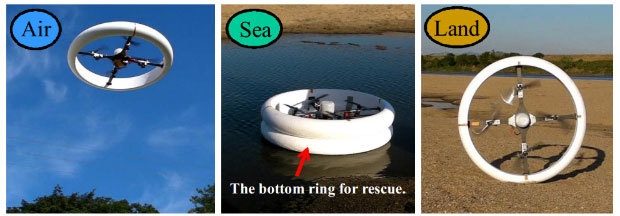
\includegraphics[width=\linewidth]{images/muwa.jpg}
  \caption{The MUWA model (courtesy of \cite{Kawasaki2013})}
  \label{fig:muwa}
\end{figure}


\begin{itemize}
    \item AQUA 
    \item MUWA  
    \item A. Crespi CPG robots
    \item Alex Kossett's hybrid air-land robot
    \item S. Mintchev and Floreano's air-land robot. 
    \item Velox Pliant Energy Systems Amphibious Robot https://www.pliantenergy.com/home-1/
\end{itemize}

